% Original book p37; original base PDF p41; input PDF p53; p037_s08 一、8
% Role: answer; original field: answer_latex
% Compile with XeLaTeX from this figures/ directory.
\documentclass[12pt,tikz,border=5pt]{standalone}
\usepackage{fontspec}
\setmainfont[Path=../fonts/]{DroidSansFallback.ttf}
\setsansfont[Path=../fonts/]{DroidSansFallback.ttf}
\usepackage{amsmath,amssymb}
\usepackage{tikz}
\usetikzlibrary{calc,angles,quotes,arrows.meta,decorations.pathreplacing,decorations.pathmorphing,decorations.markings,patterns,positioning,fit,backgrounds,matrix,intersections,shapes.geometric}
\begin{document}
\color{red}
\tikzset{every picture/.append style={color=red}}
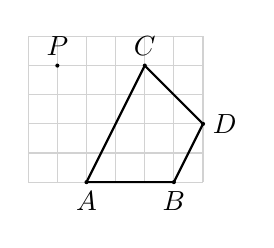
\begin{tikzpicture}[scale=.37]\draw[step=1,gray!35] (0,0) grid (6,5);\coordinate(A)at(2,0);\coordinate(B)at(5,0);\coordinate(C)at(4,4);\coordinate(D)at(6,2);\coordinate(P)at(1,4);\draw[thick](A)--(B)--(D)--(C)--cycle;\foreach \q/\lab/\pos in {A/A/below,B/B/below,C/C/above,D/D/right,P/P/above}{\fill(\q)circle(2pt)node[\pos]{$\lab$};}\end{tikzpicture}

\end{document}
